% Signals and Systems (ETH, HS26, Dr. A. Carron) -- exam cheat sheet
% FRONT SIDE: Weeks 1-5 (signals, LTI, representations, discretization, z-transform)
% BACK SIDE (todo): Weeks 6-13 (frequency domain, filter design, review)
\documentclass[a4paper]{article}
\usepackage[a4paper,margin=4.5mm,top=4mm,bottom=4mm]{geometry}
\usepackage{amsmath,amssymb,mathtools}
\usepackage{multicol}
\usepackage[dvipsnames]{xcolor}
\usepackage{enumitem}
\usepackage{array,tabularx,booktabs}
\usepackage{tikz}
\usetikzlibrary{arrows.meta,positioning}

\pagestyle{empty}
\setlength{\parindent}{0pt}
\setlength{\parskip}{0.4pt}
\setlength{\columnsep}{2.2mm}
\setlength{\columnseprule}{0.2pt}
\def\columnseprulecolor{\color{gray!60}}
\setlength{\abovedisplayskip}{1pt}
\setlength{\belowdisplayskip}{1pt}
\setlength{\abovedisplayshortskip}{0.5pt}
\setlength{\belowdisplayshortskip}{0.5pt}
\setlength{\jot}{0.5pt}
\setlength{\arraycolsep}{1.4pt}
\setlength{\tabcolsep}{1.6pt}
\renewcommand{\arraystretch}{0.95}
\setlist{nosep,leftmargin=6pt,labelsep=2pt,itemsep=0pt,topsep=0pt}
\setlist[itemize]{label=$\bullet$}
\medmuskip=2mu plus 1mu minus 2mu
\thickmuskip=3mu plus 2mu minus 2mu
\thinmuskip=1.5mu

% colours per week
\definecolor{w1}{HTML}{1F5FA8}
\definecolor{w2}{HTML}{0E7C66}
\definecolor{w3}{HTML}{8A4FB0}
\definecolor{w4}{HTML}{B5561B}
\definecolor{w5}{HTML}{B0233F}
\definecolor{gen}{HTML}{4A4A4A}

\newcommand{\wk}[2]{\par\vspace{1.2pt}\noindent\colorbox{#1}{\parbox{\dimexpr\columnwidth-2\fboxsep}{\color{white}\bfseries\strut #2}}\par\vspace{0.6pt}}
\newcommand{\sub}[2][black]{\par\vspace{0.8pt}{\color{#1}\bfseries\underline{#2}}\ }
\newcommand{\warn}[1]{{\color{red!75!black}\textbf{!}\,#1}}
\newcommand{\up}[1]{\underset{\uparrow}{#1}}
\newcommand{\T}{^{\!\top}}
\newcommand{\dd}{\,\mathrm{d}}
\newcommand{\ej}[1]{e^{j#1}}

\DeclareMathSizes{6.3}{6.3}{4.7}{3.8}
\begin{document}
\fontsize{6.3}{7.1}\selectfont\raggedright
\setlength{\abovedisplayskip}{1.5pt}\setlength{\belowdisplayskip}{1.5pt}%
\setlength{\abovedisplayshortskip}{1pt}\setlength{\belowdisplayshortskip}{1pt}%
\begin{multicols*}{4}

% =====================================================================
\wk{gen}{Math toolbox}
\textbf{Geometric:} $\sum_{k=0}^{\infty}a^k=\frac{1}{1-a}\ (|a|<1)$,\
$\sum_{k=0}^{N-1}a^k=\frac{1-a^N}{1-a}$,\
$\sum_{k\ge0}k a^k=\frac{a}{(1-a)^2}$,\
$\sum_{k\ge1}a^{k}=\frac{a}{1-a}$.\\
\textbf{Complex:} $z=a+jb=re^{j\theta}$, $r=\sqrt{a^2+b^2}$, $\theta=\operatorname{atan2}(b,a)$;
$e^{j\theta}=\cos\theta+j\sin\theta$;
$\cos\theta=\frac{e^{j\theta}+e^{-j\theta}}{2}$, $\sin\theta=\frac{e^{j\theta}-e^{-j\theta}}{2j}$;
$\frac1z=\frac{\bar z}{|z|^2}$; $|z_1z_2|=|z_1||z_2|$, $\angle(z_1z_2)=\angle z_1+\angle z_2$;
$e^{j\pi}=-1$, $e^{j\pi/2}=j$; angles mod $2\pi$.\\
\textbf{2$\times$2:} $A=\begin{bsmallmatrix}a&b\\c&d\end{bsmallmatrix}$:
$A^{-1}=\frac{1}{ad-bc}\begin{bsmallmatrix}d&-b\\-c&a\end{bsmallmatrix}$,\
$\det(zI-A)=z^2-\operatorname{tr}(A)z+\det A$,\
$\lambda_{1,2}=\tfrac{\operatorname{tr}}{2}\pm\sqrt{\tfrac{\operatorname{tr}^2}{4}-\det}$.
Triangular $\Rightarrow$ eigenvalues on diagonal.\\
\textbf{Taylor:} $e^x=\sum\frac{x^k}{k!}$, $\sin x\approx x$, $\cos x\approx 1-\frac{x^2}{2}$, $\sqrt{q}\approx\sqrt{q_e}+\frac{\Delta q}{2\sqrt{q_e}}$.

% =====================================================================
\wk{w1}{W1 \ Signals \& system properties}
\sub[w1]{Signals} CT $x(t),t\!\in\!\mathbb R$; DT $x[n],n\!\in\!\mathbb Z$ (sequence). $\{x[n]\}$ = whole signal. Arrow $\uparrow$ marks $n=0$; unlisted samples $=0$.\\
$\{2,\up{3},1\}$: $x[-1]=2,\ x[0]=3,\ x[1]=1$.
\sub[w1]{Operations} (compose in any order)\\
$\alpha x[n]$ scaling;\ \ $x[n-k]$ ($k>0$) \textbf{delay} = shift \textbf{right};\ \ $x[n+k]$ \textbf{advance} = shift \textbf{left};\ \ $x[-n]$ reversal about $n=0$.\\
Locate sample: set argument $=$ index, e.g.\ $x[n-2]$ has $x[0]$ at $n=2$.\\
$x[-n+k]=x[-(n-k)]$: \emph{first} flip, \emph{then} delay by $k$.
\sub[w1]{Key signals} $\delta[n]=1$ for $n=0$, else $0$; \ $s[n]=1$ for $n\ge0$, else $0$.\\
$s[n]=\sum_{k=-\infty}^{n}\delta[k]$,\quad $\delta[n]=s[n]-s[n-1]$\\
$x[n]\delta[n-k]=x[k]\delta[n-k]$ (sifting)\\
\textbf{Impulse decomposition:} $x[n]=\sum_{k}x[k]\,\delta[n-k]$\\
e.g.\ $\{\up1,2\}=\delta[n]+2\delta[n-1]$.\\
\textbf{Causal signal:} $x[n]=0\ \forall n<0$ ($\ne$ causal system!).\\
\textbf{Bounded:} $\exists M<\infty:\ |x[n]|\le M\ \forall n$.
\sub[w1]{System} $y=G\,u$. Properties (prove with the definition; disprove with \emph{one} counterexample):\\
\begin{tabularx}{\columnwidth}{@{}l>{\raggedright\arraybackslash}X@{}}
\textbf{Memoryl.} & $y[n]$ depends only on $u[n]$\\
\textbf{Causal} & $y[n]$ depends only on $u[k],\,k\le n$\\
\textbf{Linear} & $G\{\alpha_1u_1{+}\alpha_2u_2\}=\alpha_1y_1{+}\alpha_2y_2$ $\forall u_i,\alpha_i$\\
\textbf{TI} & $u_1[n{-}k]\mapsto y_1[n{-}k]\ \forall k$\\
\textbf{BIBO} & $|u[n]|\le1\,\forall n\Rightarrow |y[n]|\le M<\infty$
\end{tabularx}
\textbf{TI test:} compute $y_2[n]=G\{u_1[n-k]\}$ and compare with $y_1[n-k]$ (replace \emph{every} $n$ by $n-k$).\\
\textbf{Quick tells:}
\begin{itemize}
\item Linear $\Rightarrow0\mapsto0$. $u{+}2$, $u^2$, $\cos u$, $u[n]u[n{-}1]$: \emph{not} linear (affine $\ne$ linear).
\item Explicit $n$ ($n\,u[n]$, $s[n]u[n]$), $u[2n]$, $u[-n]$: \emph{not} TI. $g[n]u[n]$: linear $\forall g$.
\item $u[n{+}k]$, $u[-n]$: \emph{not} causal. $\cos u$: memoryless, stable, nonlinear.
\item $n\,u[n]$ unstable ($u{=}s\Rightarrow y{=}ns[n]$); $y[n]{=}a y[n{-}1]{+}u[n]$ stable iff $|a|{<}1$.
\end{itemize}

% =====================================================================
\wk{w2}{W2 \ Impulse response \& convolution}
$h[n]:=G\{\delta[n]\}$. For \textbf{LTI}: $\delta[n-k]\mapsto h[n-k]$ (TI), $c\,\delta[n-k]\mapsto c\,h[n-k]$ (L) $\Rightarrow$ $h$ determines $G$ completely.\\
\textbf{Convolution} (needs L \emph{and} TI):
\[y[n]=\textstyle\sum_{k}u[k]\,h[n{-}k]=\sum_k h[k]\,u[n{-}k]\]
\textbf{By hand:} flip $h$, slide, multiply overlap, sum; or $y[n]=\sum_{i+j=n}u[i]h[j]$ (polynomial product).\\
\textbf{Support:} lengths $L_y=L_u+L_h-1$; start index $n_u+n_h$, end index $e_u+e_h$.\\
\textbf{Check:} $\sum_n y[n]=\big(\sum u\big)\big(\sum h\big)$.\\
Ex: $\{\up1,2,3\}*\{\up1,\tfrac12\}=\{\up1,\tfrac52,4,\tfrac32\}$; $\{\up1,-1,2\}*\{\up1,1,1\}=\{\up1,0,2,1,2\}$.
\sub[w2]{Properties}
commutative $u*h=h*u$; associative $(u*h_1)*h_2=u*(h_1*h_2)$; distributive $u*(h_1+h_2)=u*h_1+u*h_2$;
identity $u*\delta=u$; shift $u*\delta[n-k]=u[n-k]$; \warn{$u*h\neq u\cdot h$.}\\
\textbf{Interconnections:} series $\Rightarrow h_1*h_2$ (order irrelevant for LTI); parallel $\Rightarrow h_1+h_2$; direct path $\Rightarrow+\delta$.
E.g.\ $\delta+\{\up1,-1\}*\{\up1,1\}=\{\up2,0,-1\}$.\\
\textbf{Deconvolution} ($h[0]\ne0$): solve recursively, $u[n]=\big(y[n]-\sum_{k\ge1}h[k]u[n-k]\big)/h[0]$.
\sub[w2]{Step response}
$r[n]=G\{s[n]\}=\sum_{k=-\infty}^{n}h[k]$,\quad $h[n]=r[n]-r[n-1]$.\\
Steady state (stable): $r[\infty]=\sum_k h[k]=H(1)$.
\sub[w2]{Criteria for LTI}
\textbf{Causal} $\iff h[n]=0\ \forall n<0$.\
\textbf{Memoryless} $\iff h[n]=c\,\delta[n]$.\\
\textbf{BIBO stable} $\iff \sum_k|h[k]|<\infty$ \ (then $|y|\le\sum|h|\cdot\max|u|$).
\begin{itemize}
\item $\alpha^n s[n]$: $\sum=\frac1{1-|\alpha|}$, stable iff $|\alpha|<1$.
\item $s[n]$: causal, bounded, \emph{unstable} ($u=s\Rightarrow y=(n{+}1)s[n]$).
\item $\frac{1}{n+1}s[n]$: $h\to0$ but harmonic sum diverges $\Rightarrow$ unstable. Decay/boundedness are \emph{not} enough.
\item $2^n$ for $n\le0$: $\sum=2$ $\Rightarrow$ stable, not causal (support matters, not base).
\item Cascade $s*(\delta[n]-\delta[n-1])=\delta$: unstable subsystem can be cancelled (pole-zero cancellation).
\end{itemize}
\textbf{FIR} (causal): $h[n]=0\ \forall n\ge N$ $\Rightarrow$ always stable. \textbf{IIR}: infinitely many nonzero $h[n]$ (stable or not).

% =====================================================================
\wk{w3}{W3 \ System representations}
\begin{tabular}{@{}lll@{}}
$h[n]$ & convolution & analysis\\
LCCDE & recursion & real-time (DSP)\\
$(A,B,C,D)$ & state space & simulation, design
\end{tabular}
\sub[w3]{LCCDE} (LTI by def.; order $N$): $\sum_{k=0}^{N}a_ky[n{-}k]=\sum_{k=0}^{M}b_ku[n{-}k]$, $a_0\ne0$.\\
Causal recursion: $y[n]=\frac1{a_0}\big(\sum_{k=0}^{M}b_ku[n-k]-\sum_{k=1}^{N}a_ky[n-k]\big)$.\\
\textbf{LCCDE$\to h$:} iterate with $u=\delta$, $y[n]=0$ for $n<0$.
E.g.\ $y[n]-\tfrac34y[n-1]=2u[n]\Rightarrow h=2(\tfrac34)^ns[n]$.\\
\warn{Sign:} $y[n]-a\,y[n-1]$ $\Rightarrow$ ratio $+a$.\\
\textbf{$h\to$ LCCDE:} FIR: read off, $b_k=h[k]$. Sum of geometric terms: via $H(z)$ (W5).
\sub[w3]{State space (DT)}
\[q[n{+}1]{=}Aq[n]{+}Bu[n],\ y[n]{=}Cq[n]{+}Du[n]\]
$A_{N\times N}$ dynamics, $B_{N\times1}$ input, $C_{1\times N}$ output, $D$ feedthrough ($u[n]\to y[n]$ directly). State = memory: everything from the past that still affects the future; $N$ = order (one per energy store/stored past value; inputs are \emph{not} states).
\sub[w3]{SS $\to h$} ($q[0]=0$, $u=\delta$; $q[n]=A^{n-1}B$)
\[h=\{\up{D},\,CB,\,CAB,\,CA^2B,\dots\}\]i.e.\ $h[0]=D$, $h[n]=CA^{n-1}B$ for $n\ge1$.\\
\warn{$h[0]=D$, not $CB$.} $D=0$ $\Rightarrow$ response 1 sample late.\\
Ex: $(\tfrac13,1,2,1)\Rightarrow h=\{\up1,2,\tfrac23,\tfrac29,\dots\}$.\\
With initial state: $y[n]=\underbrace{CA^nq[0]}_{\text{free}}+\underbrace{(h*u)[n]}_{\text{forced}}$.
\sub[w3]{LCCDE $\to$ SS} (companion form, $a_0=1$)\\
\emph{Course form} (RHS $=b_0u[n]$ only), $q[n]=[y[n{-}N],\dots,y[n{-}1]]\T$:
$A=\begin{bsmallmatrix}0&1&\cdots&0\\\vdots&&\ddots&\vdots\\0&0&\cdots&1\\-a_N&-a_{N-1}&\cdots&-a_1\end{bsmallmatrix}$, $B=\begin{bsmallmatrix}0\\\vdots\\0\\b_0\end{bsmallmatrix}$, $C=[-a_N\,\cdots\,-a_1]$, $D=b_0$.\\
\emph{General} (delayed inputs, $M\le N$, pad $b_k=0$): same $A$, $B=[0\cdots0\ 1]\T$,
$C=[\,b_N{-}a_Nb_0,\ \dots,\ b_1{-}a_1b_0\,]$, $D=b_0$.\\
1st order: $y[n]+a_1y[n{-}1]=b_0u[n]+b_1u[n{-}1]$: $(A,B,C,D)=(-a_1,\,1,\,b_1{-}a_1b_0,\,b_0)$.\\
Or choose state $q[n]=[y[n{-}1],u[n{-}1]]\T$ (store past inputs too).
\sub[w3]{SS $\to$ LCCDE}
Eliminate $q$ (write equation one step earlier, subtract) or via $H(z)=C(zI-A)^{-1}B+D$.
Scalar: $y[n]-A\,y[n{-}1]=D\,u[n]+(CB-AD)\,u[n{-}1]$.\\
Ex: $(\tfrac14,1,\tfrac34,1)$: $y[n]-\tfrac14y[n{-}1]=u[n]+\tfrac12u[n{-}1]$.
\sub[w3]{Non-uniqueness} $q'=Tq$ ($T$ invertible): $(TAT^{-1},\,TB,\,CT^{-1},\,D)$ gives the same $h$. Compare realizations via $h$ (or $H(z)$), \emph{never} entrywise.
E.g.\ $(\tfrac12,1,\tfrac12,1)\equiv(\tfrac12,2,\tfrac14,1)$.
\sub[w3]{CT state space}
\[\dot q=A_cq{+}B_cu,\ \ y=C_cq{+}D_cu\]
Build: first rows = definitions ($\dot q_1{=}q_2$), last row = law solved for highest derivative.\\
\textbf{MSD} $m\ddot p+c\dot p+kp=F$, $q=[p,\dot p]\T$:
$A_c=\begin{bsmallmatrix}0&1\\-k/m&-c/m\end{bsmallmatrix}$, $B_c=\begin{bsmallmatrix}0\\1/m\end{bsmallmatrix}$, $C_c=[1\ 0]$ (pos.) or $[0\ 1]$ (vel.), $D_c=0$.\\
\textbf{RC}: $RC\dot y+y=u$: $A_c=-\tfrac1{RC}$, $B_c=\tfrac1{RC}$.\
\textbf{RLC} $q=[v_C,i]\T$:
$A_c=\begin{bsmallmatrix}0&1/C\\-1/L&-R/L\end{bsmallmatrix}$, $B_c=\begin{bsmallmatrix}0\\1/L\end{bsmallmatrix}$.
\sub[w3]{Linearization}
Nonlinear $\dot q=f(q,u)$, $y=h(q,u)$.\\
1.\ \textbf{Equilibrium} $(q_e,u_e)$: $0=f(q_e,u_e)$, $y_e=h(q_e,u_e)$ (input need not be 0; may be several).\\
2.\ \textbf{Jacobians at equilibrium} (row $i$ = eq.\ $i$, column $j$ = var.\ $j$):
\[A_c{=}\tfrac{\partial f}{\partial q}\big|_e,\,B_c{=}\tfrac{\partial f}{\partial u}\big|_e,\,C_c{=}\tfrac{\partial h}{\partial q}\big|_e,\,D_c{=}\tfrac{\partial h}{\partial u}\big|_e\]
3.\ \textbf{Deviations} $\Delta q=q-q_e$, $\Delta u=u-u_e$, $\Delta y=y-y_e$:\
$\Delta\dot q=A_c\Delta q+B_c\Delta u$, $\Delta y=C_c\Delta q+D_c\Delta u$.\\
LTI (constant matrices); valid only near equilibrium. \warn{No $q$, $\sin q$ left inside matrices.}\\
\textbf{Pendulum} ($\theta$ from upright): $\dot q=\begin{bsmallmatrix}x_2\\\frac gL\sin x_1-cx_2+\frac1{mL^2}u\end{bsmallmatrix}$.
$u_e=-mgL\sin\theta_0$; $A_c=\begin{bsmallmatrix}0&1\\\frac gL\cos\theta_0&-c\end{bsmallmatrix}$, $B_c=\begin{bsmallmatrix}0\\\frac1{mL^2}\end{bsmallmatrix}$.
Upright $\theta_0{=}0$: $+\tfrac gL$; hanging $\theta_0{=}\pi$: $-\tfrac gL$.\\
\textbf{Tank} $\dot q=u-2\sqrt q$, $u_e=4$: $q_e=4$, $\Delta\dot q=-\tfrac12\Delta q+\Delta u$.\\
\textbf{Drag} $\dot v=u-v^2$: equilibria $(0,0)$, $(10,100)$, \dots; $A_c=-2v_e$.

% =====================================================================
\wk{w4}{W4 \ Sampling \& discretization}
\textbf{Sampler $S$} (CT$\to$DT): $x[n]=x(nT_s)$, $f_s=\frac1{T_s}$.\\
\textbf{ZOH $H$} (DT$\to$CT): $x(t)=x[n]$ for $nT_s\le t<(n{+}1)T_s$ (staircase, not interpolation).\\
$S\circ H=\mathrm{id}$ (hold then sample); \ $H\circ S\neq\mathrm{id}$ (inter-sample info lost).\\
Sampling can lose info: $\cos(2\pi t)$, $T_s{=}1$ $\Rightarrow$ $x[n]=1$ (same as const.). $T_s{=}\frac12$: $(-1)^n$; $T_s{=}\frac14$: $\{1,0,-1,0\}$; $T_s{=}\frac13$: $\{1,-\frac12,-\frac12\}$. \ DT freq.\ $\Omega=\omega T_s$.
\sub[w4]{Hold-and-sample architecture}
\par\vspace{1pt}\centerline{%
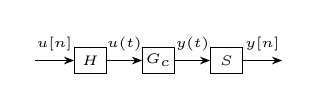
\begin{tikzpicture}[font=\tiny,node distance=4.5mm,>={Stealth[length=1.3mm]},
  b/.style={draw,minimum height=3.2mm,minimum width=4mm,inner sep=1pt}]
\node[b](H){$H$};\node[b,right=of H](G){$G_c$};\node[b,right=of G](S){$S$};
\draw[->](H.west)++(-5mm,0)--node[above]{$u[n]$}(H.west);
\draw[->](H)--node[above]{$u(t)$}(G);\draw[->](G)--node[above]{$y(t)$}(S);
\draw[->](S.east)--node[above]{$y[n]$}++(5mm,0);
\end{tikzpicture}}\par\vspace{1pt}
$G_d=S\,G_c\,H$ (composition read right-to-left). $u[n],y[n]$ DT; $u(t),y(t)$ CT.\\
Pure delay plant $y(t)=u(t-\tau)$, $kT_s<\tau\le(k{+}1)T_s$ $\Rightarrow$ $y[n]=u[n-k-1]$ (rounded \emph{up}); $\tau=0\Rightarrow y[n]=u[n]$.
\sub[w4]{Euler forward} $\dot q\approx\frac{q(t+T_s)-q(t)}{T_s}$
\[A_d=I+T_sA_c,\quad B_d=T_sB_c\]$C_d=C_c$, $D_d=D_c$ (no derivative in output eq.). 
Error $\mathcal O(T_s^2)$/step. \textbf{Stability:} need $|1+T_s\lambda_i|<1$ $\forall$ eig.\ $\lambda_i$ of $A_c$.
Scalar $a<0$: stable iff $T_s<\frac{2}{|a|}$; monotone iff $T_s<\frac1{|a|}$; $\frac1{|a|}<T_s<\frac2{|a|}$: decays but alternates sign (fake oscillation).
Ex: $\dot q=-4q+u$, $T_s=0.2$: $a_d=0.2$, $b_d=0.2$.\\
\warn{Common errors: forgetting $I$, sign, discretizing $C,D$.}
\sub[w4]{Exact (ZOH) discretization}
Input constant on each interval $\Rightarrow$ augment $r=[q;u]$:
\[M=\begin{bmatrix}A_c&B_c\\0&0\end{bmatrix},\quad e^{MT_s}=\begin{bmatrix}A_d&B_d\\0&I\end{bmatrix}\]
$A_d=e^{A_cT_s}$ (top-left), $B_d$ = top-right block, $C_d=C_c$, $D_d=D_c$. Exact at sampling instants.\\
Equivalently $B_d=\int_0^{T_s}e^{A_c\tau}\dd\tau\,B_c=A_c^{-1}(A_d-I)B_c$ ($A_c$ invertible).\\
\textbf{Scalar:} $a_d=e^{aT_s}$,\ $b_d=\frac{b}{a}\big(e^{aT_s}-1\big)$ \ ($a=0$: $b_d=bT_s$).\\
\textbf{Eigenvalues:} $\lambda\mapsto e^{\lambda T_s}$, $|e^{\lambda T_s}|=e^{\operatorname{Re}\lambda\,T_s}$ $\Rightarrow$ CT stable $\Rightarrow$ DT stable for \emph{every} $T_s$. Stable 1st order: $0<a_d<1$.\\
\begin{tabular}{@{}lll@{}}\toprule
&Euler&Exact\\\midrule
$A_d$&$I+T_sA_c$&$e^{A_cT_s}$\\
$B_d$&$T_sB_c$&top-right of $e^{MT_s}$\\
accuracy&$\mathcal O(T_s^2)$&exact (ZOH)\\
stability&small $T_s$ only&always kept\\\bottomrule
\end{tabular}\\
Fast dynamics / large $T_s$ $\Rightarrow$ exact; slow \& small $T_s$ $\Rightarrow$ Euler OK.
\sub[w4]{Matrix exponential by hand}
$e^{At}=\sum_k\frac{(At)^k}{k!}$, $\frac{d}{dt}e^{At}=Ae^{At}$, $e^{0}=I$.
\begin{itemize}
\item Diagonal: $e^{\mathrm{diag}(\lambda_i)t}=\mathrm{diag}(e^{\lambda_it})$ (off-diag stays 0).
\item Nilpotent ($M^k=0$): series ends, e.g.\ $M^3=0$ for cart.
\item Diagonalizable $A=V\Lambda V^{-1}$: $e^{At}=Ve^{\Lambda t}V^{-1}$.
\item $\begin{bsmallmatrix}\lambda&1\\0&\lambda\end{bsmallmatrix}$: $e^{\lambda t}\begin{bsmallmatrix}1&t\\0&1\end{bsmallmatrix}$;\
$\begin{bsmallmatrix}\sigma&\omega\\-\omega&\sigma\end{bsmallmatrix}$: $e^{\sigma t}\begin{bsmallmatrix}\cos\omega t&\sin\omega t\\-\sin\omega t&\cos\omega t\end{bsmallmatrix}$
\item Scalar block pattern: $M^k=\begin{bsmallmatrix}a^k&a^{k-1}b\\0&0\end{bsmallmatrix}$.
\end{itemize}
\textbf{Standard results:}
\begin{itemize}
\item Integrator/tank $\dot q=u$: $a_d=1$, $b_d=T_s$.
\item Leaky tank $\dot q=-q+u$: $a_d=e^{-T_s}$, $b_d=1-e^{-T_s}$ ($T_s{=}0.5$: $0.607,\,0.393$).
\item Cart $\dot p=v,\dot v=u$: $A_d=\begin{bsmallmatrix}1&T_s\\0&1\end{bsmallmatrix}$, $B_d=\begin{bsmallmatrix}T_s^2/2\\T_s\end{bsmallmatrix}$ (Euler: $B_d=[0,T_s]\T$, misses $T_s^2/2$).
\item Cart+friction $\dot v=-cv+u$: $A_d=\begin{bsmallmatrix}1&\beta\\0&e^{-cT_s}\end{bsmallmatrix}$, $B_d=\begin{bsmallmatrix}(T_s-\beta)/c\\\beta\end{bsmallmatrix}$, $\beta=\frac{1-e^{-cT_s}}{c}$.
\end{itemize}

% =====================================================================
\wk{w5}{W5 \ z-transform \& z-plane}
\textbf{Four objects:} $z_0\in\mathbb C$ (number) $\to$ $z_0^n$ (signal) $\to$ $H(z_0)$ (eigenvalue, a number) $\to$ $H(z)$ (function on ROC).\\
\textbf{Modes} $z^n=r^ne^{j\theta n}$: $r$ = growth/decay envelope, $\theta$ = phase advance per sample. $r<1$ decay, $r=1$ sustained, $r>1$ growth; $z=1$: const., $z=-1$: $(-1)^n$.\\
$e^{j\Omega n}$ periodic $\iff\frac{\Omega}{2\pi}=\frac mN\in\mathbb Q$; $N$ = period if $\frac mN$ irreducible.\\
\textbf{Eigenfunction:} $u[n]=z_0^n\Rightarrow y[n]=H(z_0)\,z_0^n$ with $H(z_0)=\sum_kh[k]z_0^{-k}$ (if it converges).
\sub[w5]{Definition} $X(z)=\sum_{n=-\infty}^{\infty}x[n]\,z^{-n}$, $z\in$ ROC. $H(z)=\mathcal Z\{h\}$ = transfer function; $Y=HU$.
\sub[w5]{Properties}\\
\begin{tabular}{@{}l@{\ }l@{}}
$\alpha x_1+\beta x_2$ & $\alpha X_1+\beta X_2$\\
$x[n{-}k]$, $x[n{+}k]$ & $z^{-k}X$, $z^{k}X$ (zero IC)\\
$(u*h)[n]$ & $U(z)H(z)$\\
$a^nx[n]$ & $X(z/a)$\\
$n\,x[n]$ & $-z\,\frac{d}{dz}X(z)$\\
$x[-n]$ & $X(1/z)$\\
$\sum_{k\le n}x[k]$ & $\tfrac{z}{z-1}X(z)$\\
IVT (causal) & $x[0]=\lim_{z\to\infty}X(z)$\\
FVT (if exists) & $x[\infty]=\lim_{z\to1}(z{-}1)X(z)$\\
\end{tabular}
\sub[w5]{Pairs} (causal: ROC $|z|>$ largest pole)\\
\begin{tabular}{@{}ll@{}}
$\delta[n]$ / $\delta[n-k]$ & $1$ / $z^{-k}$\\
$s[n]$ & $\frac{z}{z-1}$\\
$a^ns[n]$ & $\frac{z}{z-a}=\frac{1}{1-az^{-1}},\ |z|>|a|$\\
$-a^ns[-n-1]$ & $\frac{z}{z-a},\ |z|<|a|$ (left-sided)\\
$a^{n-1}s[n-1]$ & $\frac{1}{z-a}$\\
$n\,a^ns[n]$ & $\frac{az}{(z-a)^2}$\quad ($ns[n]\!:\frac{z}{(z-1)^2}$)\\
$(n{+}1)a^ns[n]$ & $\frac{z^2}{(z-a)^2}$\\
$r^n\cos(\theta n)s[n]$ & $\frac{z(z-r\cos\theta)}{z^2-2r\cos\theta\,z+r^2}$\\
$r^n\sin(\theta n)s[n]$ & $\frac{r\sin\theta\,z}{z^2-2r\cos\theta\,z+r^2}$
\end{tabular}\\
\warn{Expression alone is not unique: need ROC or causality.}\\
\textbf{ROC rules:} never contains poles; right-sided (causal) $\Rightarrow$ $|z|>\max|p_k|$; left-sided $\Rightarrow$ $|z|<\min|p_k|$; two-sided $\Rightarrow$ annulus; causal FIR $\Rightarrow$ all $z\ne0$. Stable (any LTI) $\iff$ ROC $\ni$ unit circle.
\sub[w5]{Obtaining $H(z)$}
\textbf{LCCDE} (delay $\to z^{-k}$):
\[H(z)=\tfrac{b_0+\dots+b_Mz^{-M}}{1+a_1z^{-1}+\dots+a_Nz^{-N}}\]
then multiply num.\ \& den.\ by $z^{\max(N,M)}$. Ex: $y[n]=\tfrac13y[n{-}1]+u[n]-u[n{-}1]\Rightarrow H=\frac{z-1}{z-1/3}$.\\
\textbf{State space:} $zQ=AQ+BU$ $\Rightarrow$
\[H(z)=C(zI-A)^{-1}B+D\]with $(zI{-}A)^{-1}=\frac{\mathrm{adj}(zI-A)}{\det(zI-A)}$. 
Poles $\subseteq$ eigenvalues of $A$ (an eigenvalue may cancel with a zero).
Ex: $(\tfrac12,1,\tfrac12,1)$: $\frac{1/2}{z-1/2}+1=\frac{z}{z-1/2}$.
\sub[w5]{Poles \& zeros}
$H(z)=b_0z^{N-M}\frac{(z-z_1)\cdots(z-z_M)}{(z-p_1)\cdots(z-p_N)}$; zeros $\circ$ (num.\ roots), poles $\times$ (den.\ roots). $N>M$: zeros at $0$; $M>N$: poles at $0$.
\sub[w5]{Inverse via partial fractions}
Expand $\frac{H(z)}{z}=\frac{d}{z}+\sum_k\frac{c_k}{z-p_k}$, \ $c_k=\big[(z-p_k)\tfrac{H(z)}{z}\big]_{z=p_k}$, $d=H(0)$:
\[H(z)=d+\textstyle\sum_k\frac{c_kz}{z-p_k}\]\[\Rightarrow\ h[n]=d\,\delta[n]+\textstyle\sum_kc_k\,p_k^n\,s[n]\]
One mode $p_k^n$ per pole; weights from numerator. Ex: $\frac{z^2}{(z-\frac12)(z-\frac14)}=\frac{2z}{z-\frac12}-\frac{z}{z-\frac14}\Rightarrow h=\big(2(\tfrac12)^n-(\tfrac14)^n\big)s[n]$.\\
Complex pair $p,\bar p$: $c\,p^n+\bar c\,\bar p^n=2|c|\,r^n\cos(\theta n+\angle c)$.
\sub[w5]{Stability \& pole locations}
\textbf{Causal LTI: BIBO stable $\iff$ all poles strictly inside unit circle} ($|p_k|<1$) $\iff$ ROC contains $|z|=1$. SS: all $|\lambda_i(A)|<1$ (sufficient). Zeros irrelevant for stability.\\
Mode of $p=re^{j\theta}$: $\propto r^n\cos(\theta n)$. $0{<}p{<}1$ monotone decay (faster as $r\to0$); $-1{<}p{<}0$ alternating decay; $re^{\pm j\theta}$, $r{<}1$ decaying oscill.; $|p|{=}1$ sustained (tone), $p{=}1$ constant; $|p|{>}1$ diverges. $r$ = decay rate, $\theta$ = osc.\ freq.
\par\vspace{1pt}\centerline{
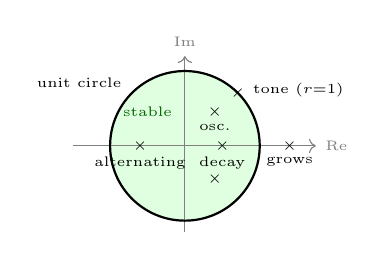
\begin{tikzpicture}[scale=0.95,font=\tiny,x=1cm,y=1cm]
\fill[green!12] (0,0) circle (1);
\draw[->,gray] (-1.5,0)--(1.75,0) node[right]{Re};
\draw[->,gray] (0,-1.15)--(0,1.2) node[above]{Im};
\draw[thick] (0,0) circle (1);
\node[anchor=east] at (-0.72,0.85) {unit circle};
\node[green!40!black] at (-0.5,0.45) {stable};
\node at (0.5,0) {$\times$}; \node[below] at (0.5,-0.02) {decay};
\node at (-0.6,0) {$\times$}; \node[below] at (-0.6,-0.02) {alternating};
\node at (0.4,0.45) {$\times$}; \node at (0.4,-0.45) {$\times$};
\node[anchor=north] at (0.4,0.42) {osc.};
\node at (0.707,0.707) {$\times$}; \node[anchor=west] at (0.78,0.75) {tone ($r{=}1$)};
\node at (1.4,0) {$\times$}; \node[below] at (1.4,-0.02) {grows};
\end{tikzpicture}}\par\vspace{1pt}
\sub[w5]{Pole placement}
Pair: $(z-re^{j\theta})(z-re^{-j\theta})=z^2-2r\cos\theta\,z+r^2$.
Envelope $\to\varepsilon$ after $N$ samples: $r=\varepsilon^{1/N}$.
Period $N_p$ samples: $\theta=\frac{2\pi}{N_p}$; in Hz: $f=\frac{\theta f_s}{2\pi}$.\\
CT pole $\lambda$ $\leftrightarrow$ DT pole $e^{\lambda T_s}$ (exact discr.).
\textbf{Workflow:} LCCDE/SS $\to H(z)\to$ poles (stability) $\to$ PFE $\to h[n]$. DC gain $=H(1)$.

\end{multicols*}
\end{document}
